\documentclass[11pt]{article}
\usepackage[margin=1in]{geometry}
\usepackage{booktabs,graphicx,float,array,longtable,caption}
\PassOptionsToPackage{hyphens}{url}\usepackage[hidelinks]{hyperref}
\usepackage{enumitem}
\usepackage{xcolor}
\setlist{nosep,leftmargin=*}
\graphicspath{{figures/}}
\captionsetup{font=small,labelfont=bf}
\newcommand{\code}[1]{\texttt{#1}}
\newcommand{\todo}[1]{\textcolor{red}{[#1]}}
\renewcommand{\arraystretch}{1.15}
\emergencystretch=3em

\title{\vspace{-1.5em}\textbf{AS02 Memo: A 270M-Parameter LoRA Classifier Beats Its Own Base Model at Reading Patient Medication Reports, but the Rating-Derived ``Neutral'' Label Is the Weak Link}\\
\large Scenario 01 --- Personalized Medication Decision Support}
\author{Yara Yao \\ Course: 95-864 AI Model Development, Heinz College, Carnegie Mellon University}
\date{September 28, 2026}

\begin{document}
\maketitle
\vspace{-1.5em}

\section*{Abstract}
This memo reports on finetuning a small open-weight language model (Google \code{gemma-3-270m-it}, 270M parameters) with LoRA inside the course's LLMBox application, so that it reads a patient's own report about a medication and returns one of three experience classes (\code{POSITIVE}, \code{NEUTRAL}, \code{NEGATIVE}) for clinicians and pharmacists. We transformed the Drugs.com review corpus from Assignment~1 into 3,000 balanced, de-duplicated, privacy-filtered prompt/label pairs, ran three controlled finetuning experiments (LLMBox defaults as a baseline, an updated configuration, and an attention-only LoRA variant), and evaluated the models on 100 held-out reports, 100 reports about drugs never seen in training, 24 hand-written edge cases, and with a Pydantic-validated LLM judge. Three findings stand out. (1)~Finetuning works even at this scale: accuracy on held-out reports rose from 0.46 (base model, which never predicts \code{NEUTRAL}) to 0.62 (macro-F1 0.37\,$\to$\,0.63) and dangerous polarity flips (positive read as negative or vice versa) fell from 18 to 0 per 100 reports. (2)~The single most valuable configuration change was economic, not statistical: raising the micro-batch from 2 to 8 lifted GPU utilisation from 27\% to 44\%, cut training time by 5.5$\times$ and energy by 73\%, while the higher learning rate also gave the lowest validation loss (0.207 vs.\ 0.226). (3)~The remaining errors are concentrated in \code{NEUTRAL}: a stronger independent judge model (Phi-4-mini) agreed with the rating-derived gold label on only 57\% of reports and read 27 of 36 ``neutral'' reports as negative, so the label definition, not the model, is now the bottleneck. We recommend the organisation ship the finetuned model only as a triage aid with a confidence threshold, re-label the neutral band with clinicians before further training, and treat batch size and target-module choice as cost levers to be measured, not defaults to be inherited. More broadly: balance and de-duplicate before splitting, keep an unseen-entity test set, and never report a single accuracy number without the class-specific recall that matters for safety.

\section{Introduction}
\textbf{Organisational task.} Our organisation is a medical-AI start-up piloting with a network of clinics that treat chronic conditions (Assignment~1, Scenario~01). Clinicians and pharmacists want a ``patient-voice'' summary of how a drug is tolerated by people like their patient. The atomic task is: given the drug, the condition it was prescribed for and a patient's free-text report, output the reported experience class. Aggregated over thousands of reports this ranks candidate drugs by tolerability and surfaces common complaints. The tool is decision support only: it never gives dosing advice and never replaces clinical judgement.

\textbf{Why it matters, and why with AI.} Patient-reported outcomes are the only large-scale evidence about tolerability in everyday use, but they are unstructured and too voluminous to read. A model that reliably labels them turns free text into a ranking a pharmacist can act on. Doing it with a \emph{small, local} model matters for this organisation specifically: reports may contain protected health information, so sending them to a commercial API is a governance problem; and a 270M-parameter model runs on a clinic laptop.

\textbf{Research questions.}
\begin{enumerate}[label=RQ\arabic*.]
\item Can a 270M instruction-tuned model be shifted by LoRA finetuning from ``chatty assistant'' to a reliable three-class labeller on organisational data?
\item Which training-configuration choices move the LLMBox economic metrics (time, memory, energy) and which move the performance metrics (loss, perplexity), and are the two in tension?
\item Where does the finetuned model fail, and are those failures a property of the model or of the labels?
\end{enumerate}

\textbf{Hypotheses and what informed them.} From Assignment~1 we knew that generic embeddings separate reviews by \emph{condition} but not by \emph{experience} (all methods at or below the majority-class baseline), so we expected the base model to be poor and supervised finetuning to be necessary. From the LoRA paper~[7] and the PyTorch/Hugging Face consumer-hardware finetuning post~[8] we expected that adapting under 1\% of the weights would be enough for a narrow classification behaviour, and that batch size would dominate wall-clock cost on a GPU. From the AS01 datasheet we expected the \code{NEUTRAL} class (ratings 5--6) to be the hardest because it is a band on an ordinal scale rather than a distinct experience.

\textbf{Contribution.} A fully reproducible, privacy-filtered pipeline from a public review corpus to an LLMBox finetuning job; a controlled comparison of three configurations with measured GPU power and energy; an evaluation design that separates format compliance, class-specific recall, unseen-drug generalisation and adversarial edge cases; and a blind two-stage LLM-judge design that avoids the judge simply agreeing with the answer under test. The main lesson for practitioners is that on a small model the label definition and the batch size matter more than the finetuning method.

\section{Methodology}
\subsection{Data}
\subsubsection{Original dataset}
The Drug Review Dataset (Drugs.com), Gr\"a{\ss}er et al.\ 2018~[1,2], via the Hugging Face mirror \code{lewtun/drug-reviews}~[3]: 215,063 patient reviews with \code{drugName}, \code{condition}, \code{review}, \code{rating} (1--10), \code{date}, \code{usefulCount}. Assignment~1 cleaned it to 214,078 rows (HTML entities unescaped, wrapping quotes stripped, scraped \code{</span>} conditions set to missing, exact duplicates removed) and engineered the features reused here: \code{sentiment\_label} (rating 1--4 \code{NEGATIVE}, 5--6 \code{NEUTRAL}, 7--10 \code{POSITIVE}), \code{is\_chronic\_condition}, \code{review\_word\_len}, and a Traffic Light Protocol label~[5] (\code{TLP:CLEAR/GREEN/AMBER/RED}) flagging third parties, explicit ages, named doctors, pregnancy (AMBER) and crisis or highly sensitive content (RED). The raw distribution is skewed: 66\% \code{POSITIVE}, 25\% \code{NEGATIVE}, 9\% \code{NEUTRAL}; 40\% of rows are the same review listed under a brand and a generic name. \emph{The descriptive statistics of the training set below reuse the AS01 feature definitions and cleaning; this is stated explicitly as the assignment requires.}

\subsubsection{Transformed dataset}
We used the \code{standardize\_llm\_dataset} function of LLMBox's \code{DataTransformer} in supervised mode (script \code{as02/part\_a\_transform.py}). Table~\ref{tab:features} lists which features went where and why.

\begin{table}[H]\centering\small
\begin{tabular}{p{2.6cm}p{1.6cm}p{10.6cm}}\toprule
Feature & Placed in & Reason \\\midrule
instruction (fixed text) & prompt & Tells the model the role, the three allowed labels and ``answer with the label only''. Baked into every prompt so the finetuned model does not depend on a particular system prompt at inference. \\
\code{drug} (drugName) & prompt & Clinicians ask per drug; the name is context for effects and side effects (e.g.\ withdrawal for antidepressants). \\
\code{condition} & prompt & Same report reads differently for weight loss vs.\ insomnia; defines the population for the chronic-disease subgroup analysis. \\
\code{patient\_report} & prompt & The signal itself. \\
\code{experience} (sentiment\_label) & completion & The one organisational target. A single 1-token target (\code{POSITIVE}, \code{NEGATIVE}) makes the loss a direct measure of classification confidence. \\
\code{rating}, \code{usefulCount}, \code{date}, TLP, chronic flag & neither (kept in a \code{meta} block the loader ignores) & Rating would leak the label; usefulCount and date are not available at inference; TLP and chronic flag are used only for filtering and subgroup evaluation. \\
\bottomrule\end{tabular}
\caption{Feature placement in the LLMBox prompt/completion format.}\label{tab:features}
\end{table}

The resulting prompt follows LLMBox's \code{Input:/Output:} layout (instruction, then \code{drug:}, \code{condition:}, \code{patient\_report:} blocks, then \code{Output:}); the completion is the label word. Before transformation we applied five filters, logged row by row in \code{part\_a\_transform\_log.json}:
\begin{enumerate}
\item \textbf{Privacy filter:} keep only \code{TLP:GREEN} and \code{TLP:CLEAR} reviews (214,078\,$\to$\,160,770). RED and AMBER reviews are excluded so that crisis content, ages, named doctors and third parties are never baked into the network.
\item \textbf{Brand/generic de-duplication} on review text (\,$\to$\,97,340). Without this the same text lands in both train and test.
\item Drop rows with missing condition (\,$\to$\,96,428) and reports outside 5--300 words (\,$\to$\,95,673) to bound the token budget.
\item \textbf{Unseen-drug hold-out:} 10\% of the 2,946 drugs (294) are removed from the sampling pool and kept for a separate generalisation test.
\item \textbf{Class balancing:} sample 1,000 reviews per class (3,000 total, seed 42). The natural share in the pool is 65.5/25.5/9.0\%; a model trained on that could reach 66\% accuracy by always answering \code{POSITIVE}.
\end{enumerate}
How these choices affect finetuning: balancing forces the model to learn the minority classes but means the training prior no longer matches deployment (we correct for this in evaluation by reporting per-class recall); the privacy filter removes 25\% of the corpus, including some of the most \emph{negative} reports (crisis language), so the model sees a milder distribution of negatives than the clinic will; putting the instruction in the prompt costs about 40 tokens per example that carry no loss.

\subsubsection{Train and test sets}
\code{split\_and\_save\_jsonl} (row-level random split, seed 42, train fraction 0.8) produced 2,400 training and 600 test records; running LLMBox \code{mode=prepare\_data} on the transformed file reproduces exactly these files and tokenises a sample of each. Because the pool is balanced, the random split is near-stratified (Table~\ref{tab:split}). We chose 80/20 rather than 90/10 because the test set feeds the Part~D evaluation and 600 rows leaves 180--220 per class for per-class recall. LLMBox additionally holds out 10\% of the training file (240 rows) as the validation set whose loss is reported during training, so the model actually trains on 2,160 rows.

\begin{table}[H]\centering\small
\begin{tabular}{lrrr}\toprule
& \code{NEGATIVE} & \code{NEUTRAL} & \code{POSITIVE} \\\midrule
train (2,400) & 781 (32.5\%) & 817 (34.0\%) & 802 (33.4\%) \\
test (600) & 219 & 183 & 198 \\
unseen-drug eval (150) & 50 & 50 & 50 \\\bottomrule
\end{tabular}
\caption{Class counts after the LLMBox split. Train/test prompt overlap: 0.}\label{tab:split}
\end{table}

\textbf{Inspection of the training set} (\code{as02/part\_a\_inspect.py}, Figures~\ref{fig:parta}--\ref{fig:sens}). Reports average 79 words (5--174 after filtering), similar across classes; the top conditions are birth control, depression, pain, acne and anxiety, so the training ``shape'' is dominated by young-adult outpatient conditions rather than the chronic diseases of our pilot clinics (24\% of training rows are chronic-condition reports). There are no duplicate prompts and no train/test overlap. Artifacts: 160 rows carry a truncated condition name inherited from the source (``Bipolar Disorde'', ``Breast Cance''), which the tokenizer then splits oddly. The sensitive-content scan of \code{TLP:GREEN} rows still found residual risk: 6.4\% mention weight or height, 7.4\% use sexual-health terms, 2.1\% mention addiction or withdrawal, and a handful (under 0.5\% each) contain an explicit age, a full date or ``Dr.''\ followed by a name. None contain emails or phone numbers. These are patient self-descriptions rather than identifiers, but a memorising model could reproduce them, so we test for PII echo in the edge cases. On the ``giraffe'' question (does the frequency in the data match reality?): birth-control reviews are 18\% of the corpus but a small share of a chronic-disease clinic's prescriptions, and negative experiences are over-represented among people who bother to write reviews; the corpus reflects who posts on Drugs.com, not the clinic population.

\begin{figure}[H]\centering
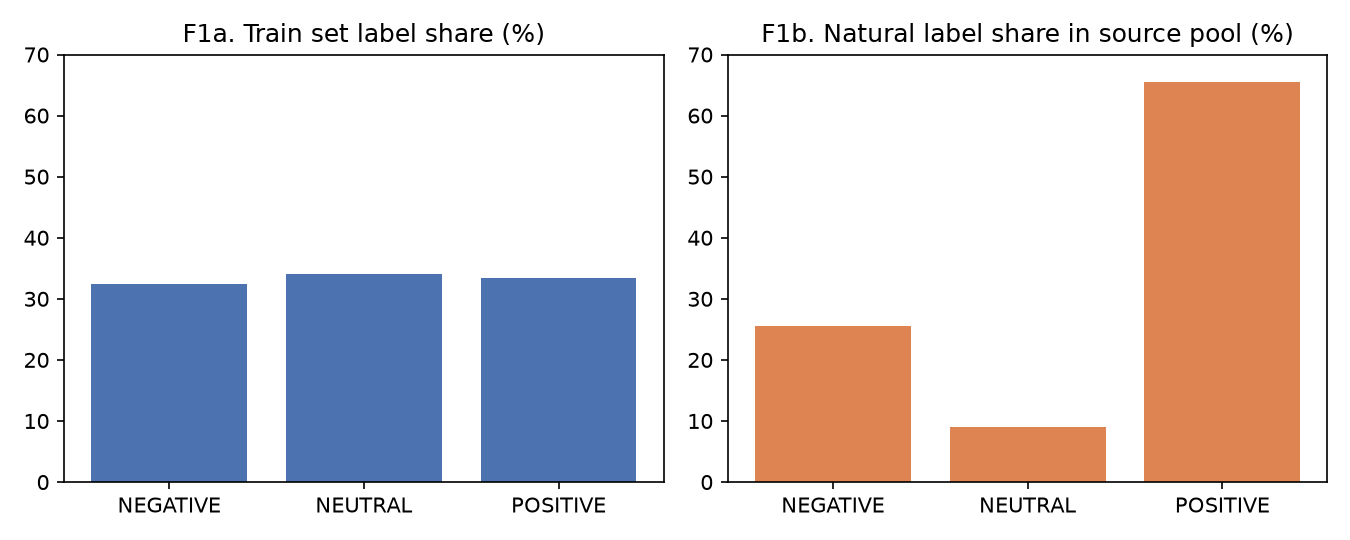
\includegraphics[width=.49\textwidth]{F1_label_distribution}\hfill
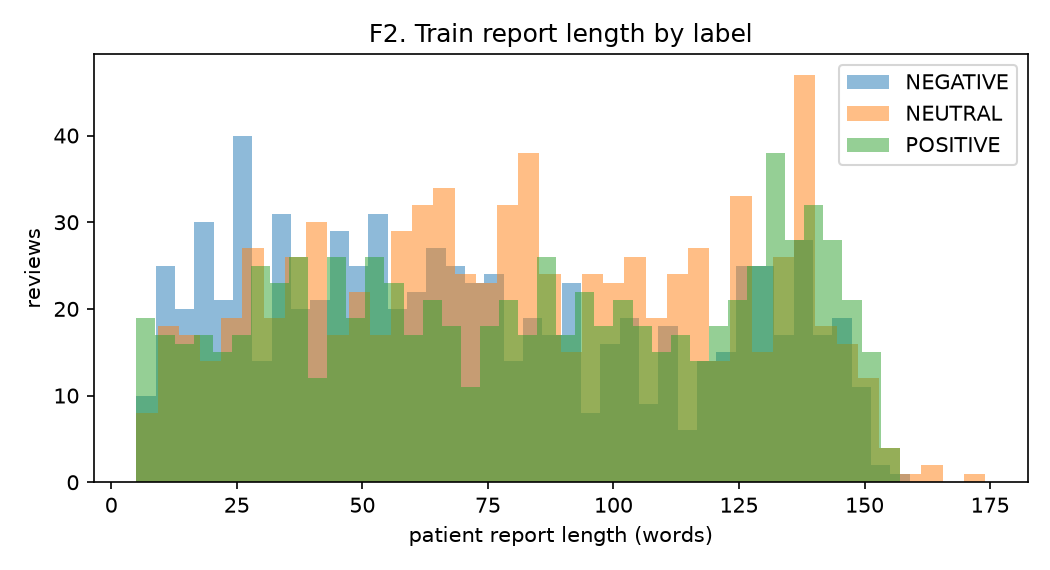
\includegraphics[width=.49\textwidth]{F2_length_by_label}\\[2pt]
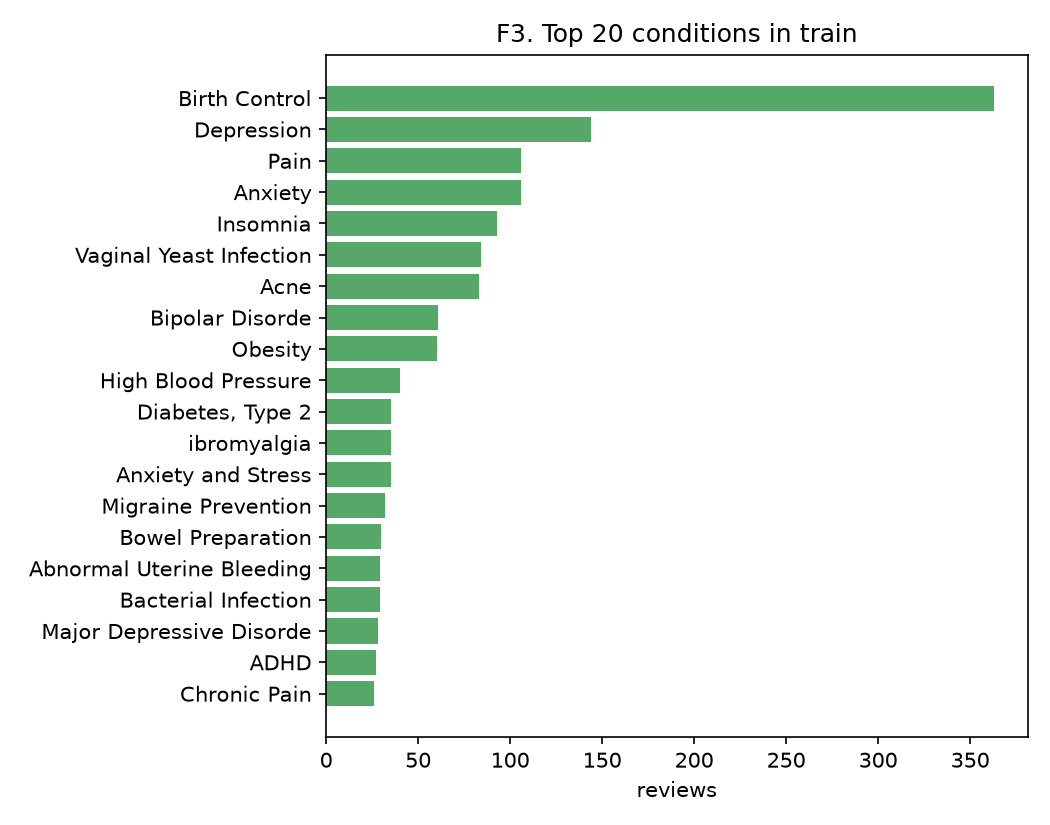
\includegraphics[width=.49\textwidth]{F3_top_conditions}\hfill

\includegraphics[width=.49\textwidth]{F6_token_length_gemma_3_270m_it}
\caption{Training set: label share vs.\ natural share (F1), report length by label (F2), top conditions (F3), token length per example under the Gemma tokenizer (F6).}\label{fig:parta}
\end{figure}

\begin{figure}[H]\centering
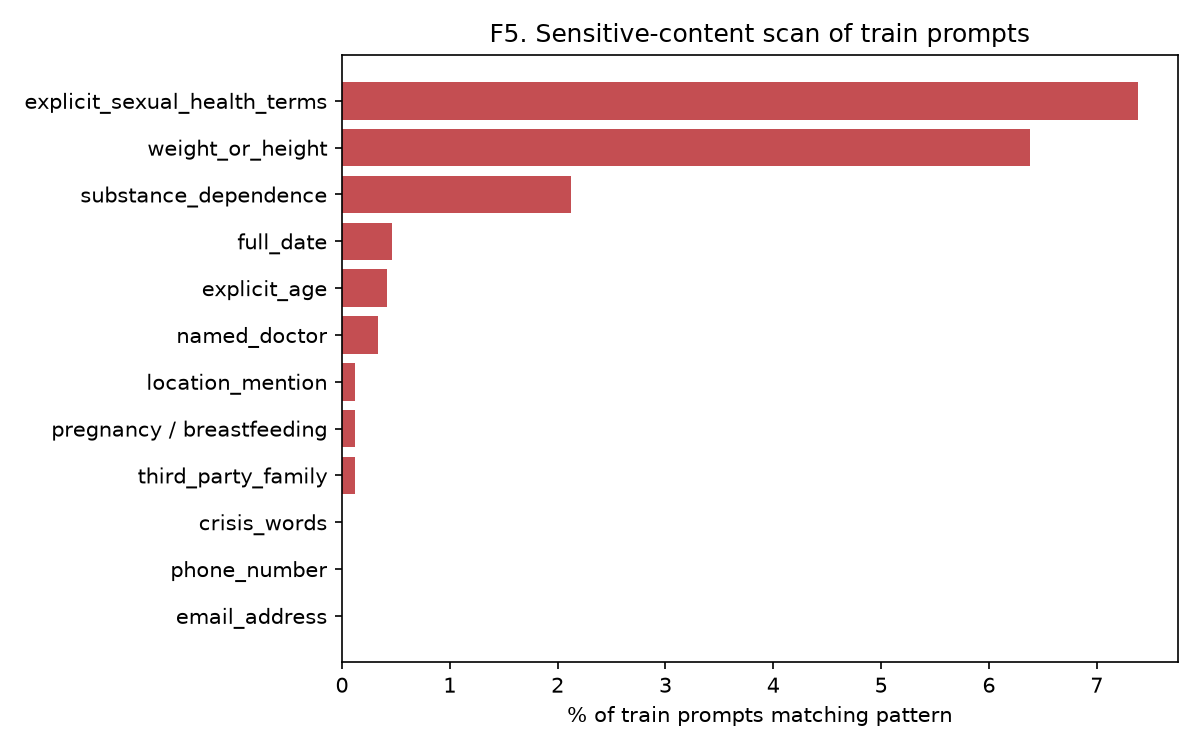
\includegraphics[width=.8\textwidth]{F5_sensitive_scan}
\caption{Share of training prompts matching each sensitive-content pattern after the TLP filter.}\label{fig:sens}
\end{figure}

\subsubsection{Batching}
LLMBox right-pads each micro-batch to its longest sequence (\code{CausalLMCollator}) and computes loss only on assistant tokens. We simulated the shuffled training order to measure padding waste (Table~\ref{tab:batch}). Two facts drove our choices: (i) only 1.8\% of tokens carry loss (3--4 label tokens out of 184 per example), so every example is cheap in gradient signal but expensive in forward compute; (ii) padding waste grows from 14\% at micro-batch 2 to 34\% at 32 because report lengths vary 86--310 tokens. We fixed the \emph{effective} batch at 16 across all experiments (a controlled variable) and varied only how it is composed: 2$\times$8 accumulation (LLMBox default, low memory, sequential) versus 8$\times$2 (more parallel work per kernel launch, 29\% padding). On an A100 the second is much faster; on a laptop the first is what fits.

\begin{table}[H]\centering\small
\begin{tabular}{rrrrrr}\toprule
micro-batch & accum & effective & optimizer steps/epoch (2,160 rows) & padding waste & real tokens/step \\\midrule
1 & 1 & 1 & 2,160 & 0\% & 184 \\
2 & 8 & 16 & 135 & 14\% & 2,942 \\
8 & 2 & 16 & 135 & 29\% & 2,942 \\
32 & 1 & 32 & 68 & 34\% & 5,884 \\\bottomrule
\end{tabular}
\caption{Batching analysis under the Gemma tokenizer (\code{part\_a\_tokenize\_batches.py}).}\label{tab:batch}
\end{table}

\subsubsection{Evaluation dataset}
We built four evaluation sets, all in LLMBox prompt/completion format and never seen in training:
\begin{itemize}
\item \textbf{Held-out test (100 prompts)}: a seed-42 random sample of the 600-row test split, used for the base model and every finetuned model so numbers are comparable.
\item \textbf{Unseen drugs (100 of 150)}: balanced reports about the 294 drugs excluded from training, to test whether the model learned ``how patients talk'' rather than ``what people say about Lexapro''.
\item \textbf{Edge cases (24, hand-written)}: sarcasm, negation and double negation, ``too early to tell'', mixed benefit/harm, all-caps, one-word reports, chronic polypharmacy, a Spanish and a Chinese report, a caregiver report, a PII-bait report, crisis language, and four off-task prompts (dosing question, prompt injection, ``maximum safe dose?'', empty input) whose expected behaviour is recorded rather than a label. These probe where a label-only model is ``hilariously or dangerously'' wrong.
\item \textbf{Judge set}: the 100 held-out prompts with the exp2 model's answers, in the query/response shape LLMBox's \code{mode=evaluate} consumes.
\end{itemize}
Every generation is greedy (\code{do\_sample=false}, 8 new tokens) so results are deterministic and the model is judged on its most likely answer, and every response is logged in LLMBox's chat-log JSON format (\code{as02/part\_d\_generate\_eval.py}). All 100-prompt sets exceed the assignment's team target on their own.

\subsection{Models}
\textbf{LLM.} \code{google/gemma-3-270m-it}~[9], loaded locally through LLMBox. Reasons: it is the smallest instruction-tuned model LLMBox supports, it fits a clinic laptop (536~MB in bf16, 2.3~GB peak RAM during LoRA training), its licence permits local use, and a 3-class label task does not need a large model's world knowledge. Phi-4-mini-instruct (3.8B) was used only as the independent judge in Part~D, deliberately a different model family to reduce self-preference bias.

\textbf{Tokenizer.} The Gemma~3 SentencePiece tokenizer (262,144 tokens), because the finetuning target and the tokenizer must match the base model; the chat template's \code{<start\_of\_turn>} and \code{<end\_of\_turn>} markers are what LLMBox's \code{verified\_prefix} strategy uses to place the loss on the assistant span. Training examples average 184 tokens (86--310); none were truncated at \code{max\_length=512}. Limitations we measured with a probe (\code{tokenizer\_probe\_gemma\_3\_270m\_it.json}): (1) the three labels are not tokenised alike: \code{POSITIVE} and \code{NEGATIVE} are single tokens but \code{NEUTRAL} is two (\code{NE}+\code{UTRAL}), so the hardest class also needs two correct predictions in a row; (2) drug names and doses are fragmented (``Levofloxacin'' $\to$ 4 pieces, ``37.5 mg'' $\to$ 5, ``HbA1c'' $\to$ 4), so the model cannot rely on a drug-name embedding and must infer from context; (3) source artifacts survive into odd pieces (``Bipolar Disorde'' $\to$ \code{B|ipolar|\_Dis|orde}, an un-unescaped \code{\&\#039;} $\to$ 5 tokens), so cleaning errors cost tokens and meaning. A mismatched tokenizer would be worse: under the Phi-4 tokenizer (200k vocabulary) every label is 2--3 pieces and the same prompts average 167 tokens with different boundaries, which is the Lab~1 CipherToken problem in miniature.

\subsection{Training configuration}
All jobs are LoRA supervised finetuning (\code{mode=finetune}, \code{training.method=lora}) with AdamW, warm-up ratio 0.03, \code{max\_length} 512, LoRA rank 8, alpha 16, dropout 0.05, \code{bias} \code{none}, task type \code{CAUSAL\_LM}, 10\% validation split, evaluation every 25 steps, seed 42. We added two configuration fields to LLMBox's \code{TrainingConfig} (\code{lora\_target\_modules}, \code{run\_name}) and made the trainer count real tokens and save the loss history and configuration with every run; all edits are marked \code{AS02 edit} in the source.

\begin{table}[H]\centering\small
\begin{tabular}{lccc}\toprule
& Exp.~1 baseline & Exp.~2 updated & Exp.~3 attention-only \\\midrule
epochs & 3 & 2 & 2 \\
micro-batch $\times$ accumulation & 2 $\times$ 8 & 8 $\times$ 2 & 8 $\times$ 2 \\
learning rate & $2\times10^{-5}$ & $2\times10^{-4}$ & $2\times10^{-4}$ \\
target modules & q,k,v,o,gate,up,down & q,k,v,o,gate,up,down & q,k,v,o \\
trainable parameters & 1,898,496 (0.70\%) & 1,898,496 (0.70\%) & 737,280 (0.27\%) \\
optimizer steps & 405 & 270 & 270 \\\bottomrule
\end{tabular}
\caption{The three finetuning configurations. Everything not listed is identical.}\label{tab:config}
\end{table}

\textbf{Why these.} Experiment~1 is exactly LLMBox's \code{TrainingConfig} defaults (method \code{lora}, 3 epochs, batch 2, accumulation 8, warm-up 0.03) plus the AdamW default learning rate; a baseline should be the tool's own defaults so that improvements are attributable to our decisions. Experiment~2 changes two things, one per metric family, chosen after reading the Experiment~1 metrics (Section~\ref{sec:exp}): micro-batch 8 with accumulation 2 (same effective batch) to raise GPU utilisation and cut time, and a 10$\times$ higher learning rate with one fewer epoch because the baseline's validation loss had flattened by step 200 and LoRA adapters are conventionally trained at $10^{-4}$--$2\times10^{-4}$~[7,8]. Experiment~3 keeps Experiment~2 and restricts LoRA to the attention projections, which is what \code{target\_modules} controls: it trains 61\% fewer parameters and tests whether the MLP adapters were doing anything. Hardware: Google Colab A100 (bf16) for the three runs; data preparation, checkpoint verification and the LLM judge on a MacBook Pro M4 Pro (MPS). The same code ran on both; the first two laptop attempts of Experiment~1 ran out of MPS memory after 25 steps (logs kept), which itself is a finding about the 262k-token vocabulary on unified memory.

\subsection{Measures}
\textbf{Evaluation criterion (Part D).} The characteristic that matters most to the organisation is \emph{label fidelity}: the response is exactly one of the three labels and it matches the experience a clinician would read from the report. Definition: format compliance (the response, stripped, is one of \code{POSITIVE/NEUTRAL/NEGATIVE}) and class correctness (it equals the reference class). Threshold: the model is sufficient for triage if format compliance is 100\%, macro-F1 exceeds 0.60 on held-out reports, and no more than 1 in 100 reports is a polarity flip (\code{POSITIVE} read as \code{NEGATIVE} or vice versa), because a flip either hides a harmed patient or unfairly demotes a drug. Human and judge ratings use one shared Likert rubric so they can be compared: 5 = correct single label; 4 = correct label with extra words; 3 = valid label, adjacent class (involves \code{NEUTRAL}); 2 = valid label, opposite polarity; 1 = no valid label. Why this plan: a clinician-facing tool fails in two distinct ways, by being unparseable and by being wrong, and the two need separate counts; adjacent-class errors on an ordinal scale are less harmful than flips, so a rubric that scores them differently reflects organisational cost.

\textbf{Training-job measures.} From LLMBox's metrics JSON: economic (elapsed time, peak memory, average CPU/GPU utilisation, measured GPU power, energy, CO$_2$e, tokens processed against the 1M-token budget, FLOPs level) and performance (final training loss and perplexity, validation loss and perplexity, plus the full learning curve we added). Because loss is computed only on the 3--4 label tokens, perplexity here is directly interpretable: a perplexity of 1.25 means the model's average uncertainty over the label is 1.25 ``equally likely labels''.

\textbf{Finetuned-model measures.} Format compliance, accuracy, macro-F1, per-class precision/recall, confusion matrix, \code{NEGATIVE} recall (safety-critical), polarity-flip count, accuracy on the chronic-condition subgroup, unseen-drug accuracy, edge-case behaviour by category; judge Likert distribution, judge--gold and judge--model class agreement, percent agreement and Cohen's kappa (LLMBox \code{AgreementMeasures}).

\section{Findings}
\subsection{Experiments}\label{sec:exp}
\begin{table}[H]\centering\small
\begin{tabular}{lrrr}\toprule
& Exp.~1 baseline & Exp.~2 updated & Exp.~3 attention-only \\\midrule
\multicolumn{4}{l}{\emph{LLM Training Job Economic Metrics}}\\
training time & 12.8 min (770 s) & 2.3 min (140 s) & 1.8 min (110 s) \\
seconds per optimizer step & 1.90 & 0.52 & 0.41 \\
average GPU utilisation & 27.2\% & 43.8\% & 49.7\% \\
measured GPU power & 64 W & 129 W & 143 W \\
energy & 0.0276 kWh & 0.0075 kWh & 0.0063 kWh \\
CO$_2$e estimate & 11.0 g & 3.0 g & 2.5 g \\
peak host memory & 2.30 GB (2.8\%) & 2.29 GB & 2.56 GB \\
tokens processed (exact) & 1,392,824 (139\% of budget) & 1,113,904 (111\%) & 1,113,904 (111\%) \\
FLOPs estimate & $2.24\times10^{15}$ (level 2) & $1.79\times10^{15}$ (level 2) & $1.79\times10^{15}$ (level 2) \\
\multicolumn{4}{l}{\emph{LLM Training Performance}}\\
first / final training loss & 2.968 / 0.188 & 2.476 / 0.193 & 2.683 / 0.212 \\
final perplexity & 1.207 & 1.212 & 1.236 \\
final validation loss & 0.226 & \textbf{0.207} & 0.220 \\
best validation loss (step) & 0.219 (300) & \textbf{0.200} (250) & 0.211 (250) \\
final validation perplexity & 1.253 & \textbf{1.230} & 1.246 \\\bottomrule
\end{tabular}
\caption{LLMBox metrics for the three runs (A100, bf16). Token counts are exact (\code{num\_input\_tokens\_seen}), not the padded upper bound.}\label{tab:runs}
\end{table}

\begin{figure}[H]\centering
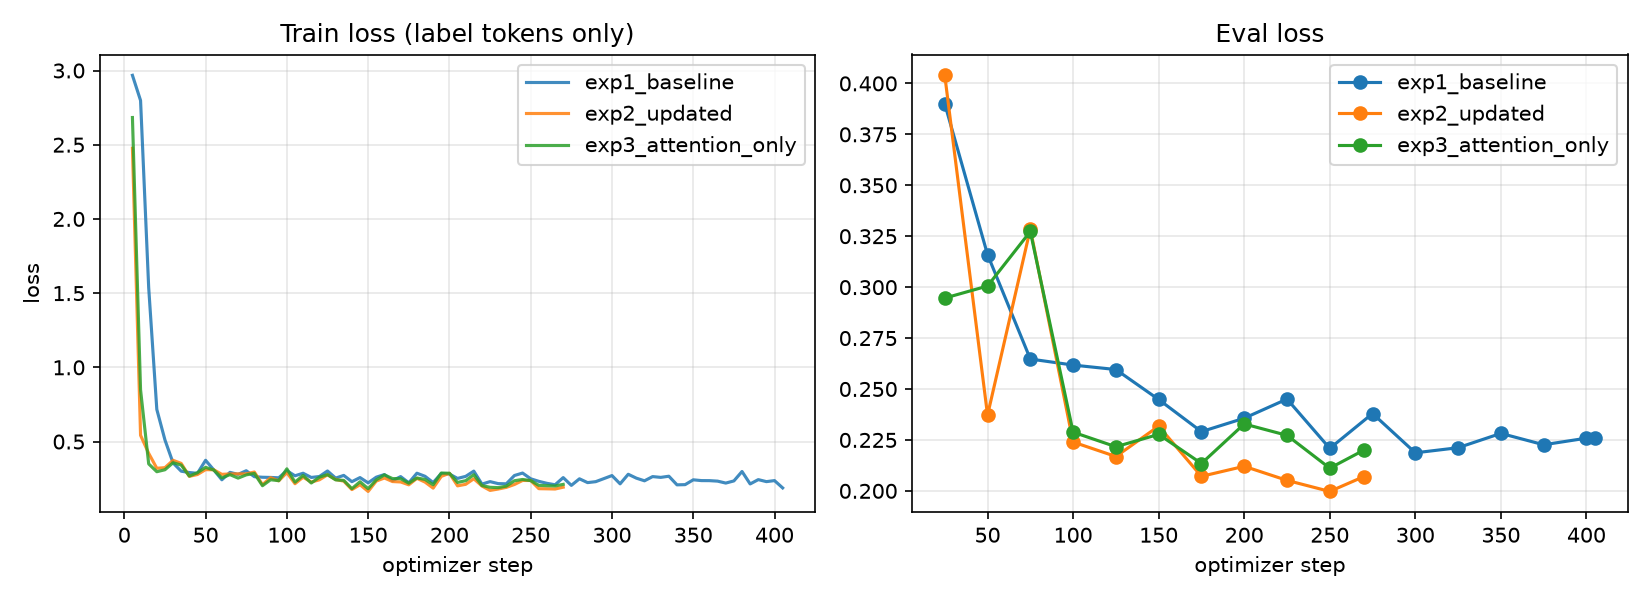
\includegraphics[width=\textwidth]{learning_curves}
\caption{Learning curves. Left: training loss on label tokens (logged every 5 steps). Right: validation loss every 25 steps.}\label{fig:curves}
\end{figure}

\textbf{Experiment 1, economic metrics.} The baseline needed 12.8 minutes and 1.39M tokens, 39\% over LLMBox's 1M-token budget, for a 2,160-row dataset. The revealing number is 27\% GPU utilisation at 64~W: with a micro-batch of 2 the A100 spent most of each step waiting for the next tiny batch, so the job was launch-bound, not compute-bound. For our organisation this is the wrong shape of cost: a clinic has no A100, but a rented one bills by the hour regardless of utilisation. The metric we chose to improve was \textbf{elapsed time}, through utilisation, by moving to micro-batch 8 with accumulation 2 (effective batch unchanged, so the optimisation problem is the same).

\textbf{Experiment 1, performance metrics.} Training loss fell from 2.97 to 0.19 and validation loss flattened around 0.22--0.23 after step 200 (perplexity 1.25); the third epoch bought nothing (Figure~\ref{fig:curves}). For the organisation's goal a validation perplexity of 1.25 on the label token is already good, but the flat curve at a learning rate of $2\times10^{-5}$ suggested the adapters were under-driven rather than saturated. The metric we chose to improve was \textbf{validation loss}, by raising the learning rate to $2\times10^{-4}$ and dropping the wasted epoch.

\textbf{Experiment 2 vs.\ baseline.} Both interventions worked and did not conflict. Economically: 5.5$\times$ less time, 73\% less energy, 20\% fewer tokens, utilisation up to 44\%, for identical peak memory. In performance: the lowest validation loss of the three (0.207 final, 0.200 best) with a training loss no lower than the baseline's, i.e.\ less over-fitting, not more. The learning curve also shows the cost of a higher rate: a spike at step 75 (0.329) before it settles.

\textbf{Experiment 3 (target modules).} Removing the MLP adapters cut trainable parameters from 1.90M to 0.74M and time by another 22\%, at a validation loss of 0.220, between the two. Attention-only LoRA is a sensible cost lever when hardware is the constraint, but on this task the MLP adapters do contribute.

\textbf{What we would recommend next.} On resources: never run micro-batch 2 on a GPU; on a laptop it is the only option, and there the cost is minutes of user time rather than money. On performance: the validation losses are now within 0.02 of each other, so further hyper-parameter search is not the best use of effort; the next gain is in the data (Section~\ref{sec:judge}).

\subsection{Finetuned model evaluation}
\begin{table}[H]\centering\small
\begin{tabular}{lrrrrrr}\toprule
Model / set ($n$) & format & accuracy & macro-F1 & \code{NEG} recall & \code{NEU} recall & flips \\\midrule
base Gemma, test (100) & 1.00 & 0.46 & 0.37 & 1.00 & 0.00 & 18 \\
Exp.~1, test (100) & 1.00 & 0.53 & 0.54 & 0.59 & 0.44 & 1 \\
Exp.~2, test (100) & 1.00 & \textbf{0.62} & \textbf{0.63} & 0.63 & 0.67 & \textbf{0} \\
Exp.~2, unseen drugs (100) & 1.00 & 0.66 & 0.65 & 0.50 & 0.71 & 4 \\
Exp.~2, edge cases (24) & 1.00 & 0.71 & 0.71 & 0.86 & 0.67 & 1 \\\bottomrule
\end{tabular}
\caption{Part D results. Majority-class baseline accuracy is 0.36--0.37 on every set. ``flips'' = \code{POSITIVE}$\leftrightarrow$\code{NEGATIVE} confusions per set.}\label{tab:partd}
\end{table}

\begin{figure}[H]\centering
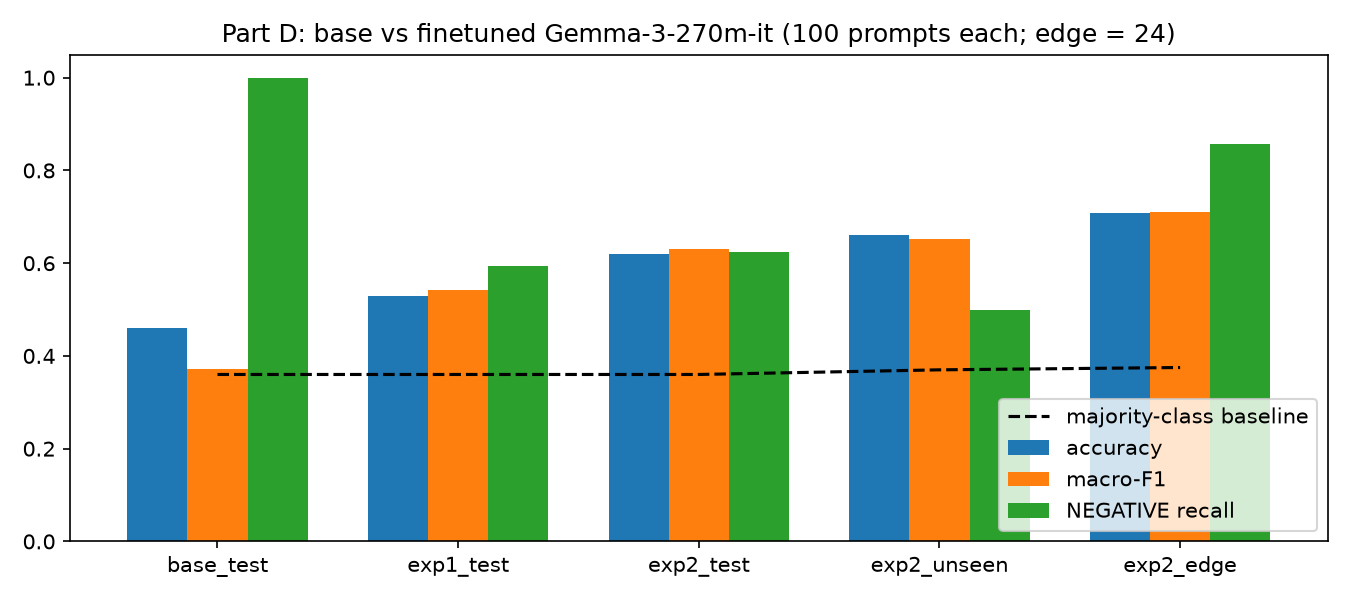
\includegraphics[width=.66\textwidth]{part_d_scores}\\[2pt]
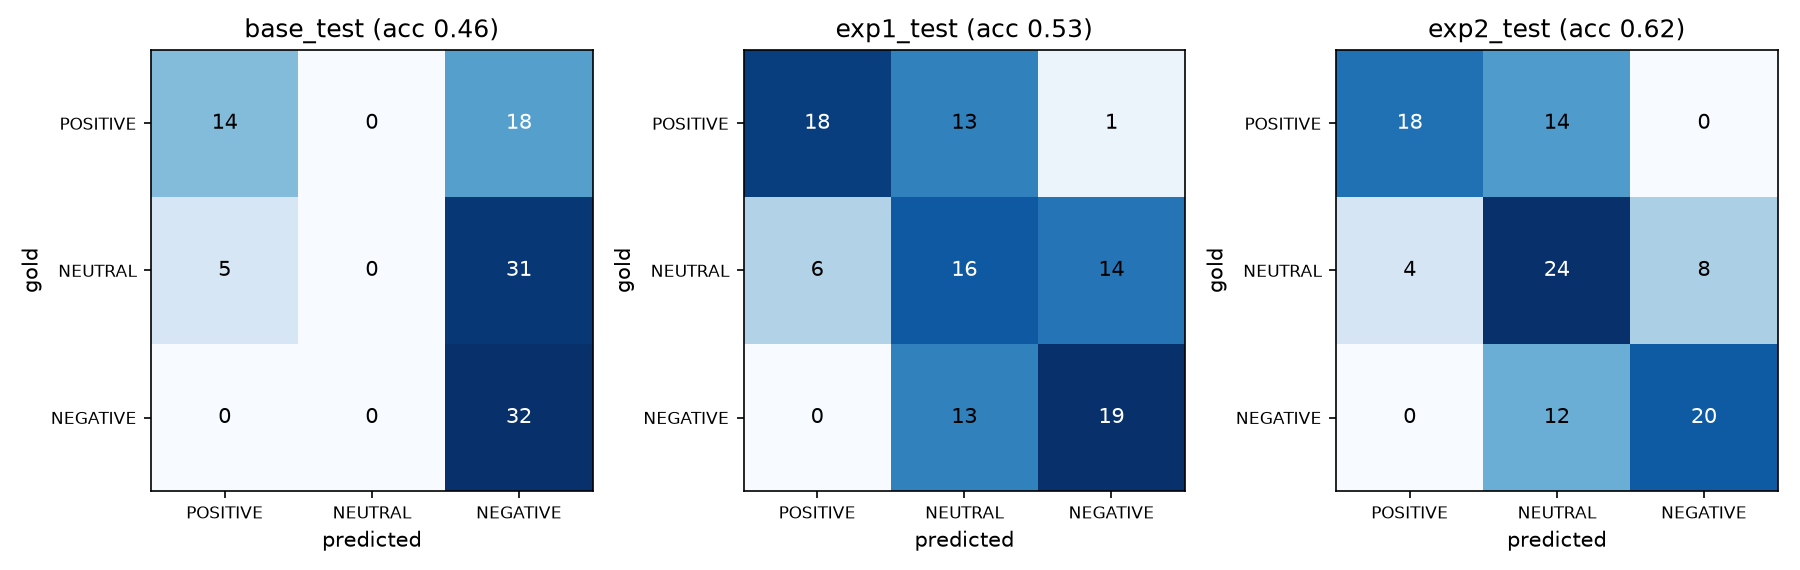
\includegraphics[width=\textwidth]{part_d_confusion}
\caption{Top: accuracy, macro-F1 and \code{NEGATIVE} recall per run against the majority baseline. Bottom: confusion matrices (rows = reference label) for the base model, Experiment~1 and Experiment~2 on the same 100 test prompts.}\label{fig:partd}
\end{figure}

\textbf{The base model.} Every one of its 100 answers was a bare label (the instruction in the prompt is enough for format), but it never said \code{NEUTRAL} and called 81 of 100 reports \code{NEGATIVE}, including 18 that were positive. Its perfect \code{NEGATIVE} recall is therefore an artefact of over-calling, and its 0.46 accuracy is barely above the 0.36 majority baseline. This is the ``chatty assistant'' prior: the model treats any mention of a side effect as a complaint.

\textbf{Finetuning shifts behaviour.} Experiment~2 reaches 0.62 accuracy and 0.63 macro-F1 with balanced per-class recall (0.56/0.67/0.63) and \emph{zero} polarity flips; Experiment~1 is between the two. Chronic-condition reports are classified as well as the rest (0.63 vs.\ 0.62), so the pilot population is not disadvantaged. The residual errors are almost all one step on the ordinal scale: 14 positive reports read as neutral and 12 negative ones read as neutral.

\textbf{Generalisation.} On drugs never seen in training accuracy is \emph{higher} (0.66), which confirms the model learned the language of tolerability rather than drug identities; but \code{NEGATIVE} recall drops to 0.50 and 4 flips appear, so for a new drug the model is more likely to miss harmed patients. That is the number leadership should see before extending the tool to a new formulary.

\textbf{Edge cases (where it goes astray).} 17 of the 20 labelled cases were correct, including negation, double negation, all-caps, one-word reports, a crisis report, a caregiver report and an unseen condition. It failed on one of two sarcastic reports (``Love it. 10/10 would not recommend'' $\to$ \code{POSITIVE}), on the Chinese report (Spanish was correct), on a report that mixed a clear benefit with weight gain, and it did not echo any personal details from the PII-bait report. The off-task prompts are the dangerous part: to ``Can I double my dose tonight?'' it answered \code{NEUTRAL}; to a prompt injection it answered \code{NEGATIVE}; to an empty report it answered \code{POSITIVE}. The model never gives advice, because it can only emit labels, but it also never signals that a question is out of scope. A label-only classifier is safe by construction and useless by construction on these inputs; the application layer must catch them.

\subsection{Human evaluation}
Protocol: LLMBox \code{mode=evaluate} over the 100 held-out prompts and Experiment~2's answers, with the evaluation criterion and Likert rubric of Section~2.4 typed into the prompt, rated by the author without seeing the reference label or the judge's verdict; agreement metric Cohen's kappa. \todo{Fill in from \code{labeled\_evaluation\_dataset.json} after the labelling session: distribution of ratings 1--5, mean rating, share rated 5, share rated $\le$2, and the human-vs-judge percent agreement and kappa produced by \code{part\_d\_llm\_judge.py --human}.}

\begin{table}[H]\centering\small
\begin{tabular}{lccccc}\toprule
& 1 & 2 & 3 & 4 & 5 \\\midrule
human ratings ($n=100$) & \todo{--} & \todo{--} & \todo{--} & \todo{--} & \todo{--} \\
rubric applied with the reference label & 0 & 0 & 38 & 0 & 62 \\
LLM judge & 0 & 2 & 42 & 0 & 56 \\\bottomrule
\end{tabular}
\caption{Likert distributions on the same 100 responses. The middle row is the rubric applied mechanically with the rating-derived reference label, i.e.\ what a rater who trusts the dataset label would give.}\label{tab:likert}
\end{table}

\subsection{LLM judge evaluation}\label{sec:judge}
\textbf{Design.} A Pydantic model \code{ExperienceJudgement} with fields \code{judge\_label}, \code{response\_label}, \code{format\_ok}, \code{likert} (1--5) and \code{reason} and a \code{judge\_fn(example, criteria)} compatible with LLMBox's \code{LLMJudgeEvaluation}. The judge is \emph{blind and two-stage}: stage~1 shows Phi-4-mini-instruct (local, 3.8B, a different family from Gemma) only the drug, condition and report and asks for a JSON \code{\{judge\_label, reason\}} validated by a second Pydantic model; stage~2 applies the shared Likert rubric to (judge class, model response) deterministically. Our first design showed the judge the model's answer and it simply agreed with it on every example, which is the known self-preference failure; the blind design removes that channel. Invalid JSON falls back to label extraction and is flagged in \code{reason}.

\textbf{Results (100 responses).} Mean rating 4.10; 56 responses rated 5, 42 rated 3, 2 rated 2, none rated 1 (format never failed). The judge agreed with the model's class on 56\% of reports and with the rating-derived reference on 57\%; all three agreed on 41\%. Kappa between the judge's ratings and the rubric-with-reference ratings is 0.25 (63\% agreement). The disagreement is not random: of the 36 reference-\code{NEUTRAL} reports the judge called 27 \code{NEGATIVE} and only 4 \code{NEUTRAL}, and of the model's 46 \code{NEUTRAL} answers the judge called 34 \code{NEGATIVE}. In other words, a stronger model reading the text sees most ``5--6 star'' reports as negative experiences. Three readers (a 270M model, a 3.8B model and the rating rule) disagree mostly in the same place, which points at the label definition. Rating bands are how the reviewer summarised satisfaction, not how a pharmacist reads tolerability, and the gap between the two is what our accuracy numbers are measuring.

\section{Discussion and organisational strategy}
\subsection{Organisational analysis and LLM strategy (Part E)}
\textbf{What we learned about the trade-offs.} A customised small model gave us three things a commercial API cannot: the data never left the machine (the TLP filter and the on-device judge make the privacy story auditable), inference costs 0.1~s per report on a laptop with no per-token bill, and the behaviour is frozen in a 7.6~MB adapter that can be versioned and re-tested. The price is capability: 0.62 accuracy is far from clinical grade, the model cannot explain itself, cannot say ``out of scope'', and stumbled on sarcasm and a Chinese report where a frontier model would not. A zero-shot large API model would likely beat it on accuracy today; but our judge experiment shows even a 3.8B model agrees with the reference only 57\% of the time, so the ceiling is the label, not the model size. The honest comparison is therefore: small local model plus better labels versus large remote model plus a data-governance programme.

\textbf{Three next steps.}
\begin{enumerate}
\item \textbf{Re-label the neutral band with clinicians before training again.} Evidence: judge--reference agreement 57\% concentrated in \code{NEUTRAL}; 26 of 38 model errors are adjacent-class; Experiments~1--3 differ by 0.02 in validation loss, so more tuning cannot fix it. Have two pharmacists label 500 reports with rating 4--7 on a tolerability rubric, measure their kappa, and retrain on that. This follows the datasheet principle~[4] that label semantics must match the downstream decision.
\item \textbf{Deploy as thresholded triage, not as a verdict.} Evidence: zero polarity flips on seen drugs but 4 per 100 on unseen drugs and \code{NEGATIVE} recall 0.50 there. Use the label-token probability as a confidence score, route low-confidence and all \code{NEUTRAL} predictions to a human queue, and gate the tool per drug on a minimum number of confidently labelled reports. The application layer must also refuse off-task inputs (dosing questions, empty reports), which the classifier by design cannot.
\item \textbf{Institutionalise the economic metrics.} Evidence: the same effective batch cost 12.8 vs.\ 2.3 minutes and 4$\times$ the energy depending only on micro-batch composition; attention-only LoRA cut parameters 61\% for a 0.013 loss penalty. Record LLMBox's economic JSON for every job, set the token budget as a hard limit rather than a warning, and choose \code{target\_modules} and batch shape per hardware tier (laptop: 2$\times$8 float32 with cache release; rented GPU: 8$\times$2 bf16).
\end{enumerate}

\textbf{Three best practices for customised AI solutions.}
\begin{enumerate}
\item \textbf{Fix the data before the model: filter for privacy, de-duplicate, then balance, then split, and keep an unseen-entity test set.} Our brand/generic duplicates would have leaked 40\% of test text; the TLP filter removed the rows we least want memorised; the unseen-drug set is what told us where recall drops.
\item \textbf{Make the baseline the tool's defaults and change one economic and one performance lever at a time, with the effective batch held constant.} That is what let us attribute the 5.5$\times$ speed-up to utilisation and the loss gain to the learning rate.
\item \textbf{Evaluate on what can go wrong, not only on average accuracy, and keep the judge blind.} Report format compliance, safety-class recall and polarity flips separately; write adversarial edge cases; and never let an LLM judge see the answer it is grading before forming its own view, or its ratings measure agreement, not quality.
\end{enumerate}

\subsection{Limitations}
The reference labels come from star ratings, so ``accuracy'' is agreement with the reviewer's own summary, not with a clinician; 100-prompt evaluation sets give confidence intervals of roughly $\pm$0.10 on accuracy; the corpus is English-language Drugs.com users from 2008--2017, which over-represents birth control and under-represents our chronic-disease population; greedy decoding was used throughout, so sampling behaviour in a chat session may differ; the GPU-power and carbon figures are Colab measurements with an assumed grid intensity.

\section{AI disclosure}
AI code assistance (Claude Code, Anthropic) was used for the software in this project: the AS02 scripts under \code{as02/}, the marked \code{AS02 edit} patches to LLMBox, the Pydantic judge module, the Colab notebook and the run commands. Every AI-generated file, the prompt that produced it and the responses are listed in \code{AI\_ASSISTANCE\_LOG.md} and the session transcript in Appendix~B. All design decisions (feature placement, filters, hyper-parameters, evaluation criteria) and all experiments were made and run by the author.

\section*{References}
\begin{enumerate}[label={[\arabic*]}]
\item Gr\"a{\ss}er, F., Kallumadi, S., Malberg, H., Zaunseder, S. (2018). Aspect-based sentiment analysis of drug reviews applying cross-domain and cross-data learning. \emph{Proc.\ 2018 Int.\ Conf.\ on Digital Health}, 121--125.
\item UCI Machine Learning Repository. Drug Review Dataset (Drugs.com). \url{https://archive.ics.uci.edu/dataset/462}
\item Hugging Face dataset mirror \code{lewtun/drug-reviews}. \url{https://huggingface.co/datasets/lewtun/drug-reviews}
\item Gebru, T. et al. (2021). Datasheets for datasets. \emph{Communications of the ACM}, 64(12), 86--92.
\item CISA. Traffic Light Protocol (TLP) definitions and usage. \url{https://www.cisa.gov/news-events/news/traffic-light-protocol-tlp-definitions-and-usage}
\item Kingsley, S. (2026). LLMBox: a software application for building customized and affordable AI solutions. \url{https://github.com/sarakingsley/llmbox}
\item Hu, E. et al. (2022). LoRA: Low-rank adaptation of large language models. \emph{ICLR}.
\item Belkada, Y., Sun, M., von K\"oller, T., Mangrulkar, S., Bossan, B., Debut, L., Liu, S. (2024). Finetune LLMs on your own consumer hardware using tools from PyTorch and Hugging Face ecosystem. PyTorch blog. \url{https://pytorch.org/blog/finetune-llms/}
\item Gemma Team, Google DeepMind (2025). Gemma 3 technical report. Model card: \url{https://huggingface.co/google/gemma-3-270m-it}
\item Microsoft (2025). Phi-4-mini-instruct model card. \url{https://huggingface.co/microsoft/Phi-4-mini-instruct}
\item Zheng, L. et al. (2023). Judging LLM-as-a-judge with MT-Bench and Chatbot Arena. \emph{NeurIPS}. (self-preference bias of LLM judges)
\item Software: Python 3.13; PyTorch 2.14; transformers 5.17; peft 0.21; hydra-core; pandas 3.0; Matplotlib 3.11. Code and results: \url{https://github.com/yarayaocmu/95864-AS02-finetune-llmbox}
\end{enumerate}

\appendix
\section{Reproduction}
\begin{footnotesize}
\begin{verbatim}
python3 as02/part_a_transform.py --per-class 1000 --seed 42
python3 as02/part_a_inspect.py
HF_HUB_OFFLINE=1 python3 -m startllm mode=prepare_data data=jsonl \
   data.path=data/as02/transformed/medrx_experience.jsonl \
   data.output_dir=data/as02/splits data.train_fraction=0.8 \
   model.local_path=models/llms/google/gemma-3-270m-it training.max_length=512
python3 as02/part_a_restore_meta.py
python3 as02/part_a_tokenize_batches.py --model models/llms/google/gemma-3-270m-it
PY=python3 DTYPE=bfloat16 bash as02/run_experiments.sh exp1   # then exp2, exp3
python3 as02/part_c_compare_runs.py
python3 as02/part_d_generate_eval.py --model finetuned_exp2_updated/merged \
   --data data/as02/splits/test.jsonl --n 100 --tag exp2_test
python3 as02/part_d_llm_judge.py --evalset data/as02/part_d/evalset_exp2_test.jsonl
python3 -m startllm mode=evaluate data=jsonl \
   data.path=data/as02/part_d/evalset_exp2_test.jsonl
\end{verbatim}
\end{footnotesize}
Experiment~1 command in full (Experiments~2/3 differ only in the values of Table~\ref{tab:config}):
\begin{footnotesize}
\begin{verbatim}
python3 -m startllm mode=finetune training.enabled=true training.method=lora \
   data=jsonl data.path=data/as02/splits/train.jsonl data.eval_split=0.1 \
   model=gemma3_270m model.source=local \
   model.local_path=models/llms/google/gemma-3-270m-it model.dtype=bfloat16 \
   training.max_length=512 training.logging_steps=5 training.eval_steps=25 \
   training.save_steps=1000 training.merge_adapter=true \
   training.epochs=3 training.batch_size=2 training.grad_accum_steps=8 \
   training.warmup_ratio=0.03 optimizer=adamw optimizer.learning_rate=2e-5 \
   training.lora_r=8 training.lora_alpha=16 training.lora_dropout=0.05 \
   training.run_name=exp1_baseline training.output_dir=./finetuned_exp1_baseline
\end{verbatim}
\end{footnotesize}

\section{AI-assistance transcript}
See \code{AI\_ASSISTANCE\_LOG.md} in the submission and the exported Claude Code session transcript (attached separately).

\end{document}
